In this section, we define two versions of the ESS and discuss various aspects of their implementation.

\subsection{Conventional ESS}
The conventional ESS discrete-time signal, $x[k]$, is given by \citep{Farina2007a}
\begin{equation}\label{eq:A5_Impulse_Response:ESS}
x[k] = \sin \left\{ \frac{\omega_1\,N}{\ln\left(\omega_2/\omega_1\right)} \cdot \left[\left(\frac{\omega_2}{\omega_1}\right)^{\frac{k}{N}}-1\right] \right\}
\end{equation}
for $k \in[0,N-1]$, where $N = F_s T$ is the total number of samples of the signal, $T$ is the sweep duration in seconds, $F_s$ is the sampling rate in samples/second, and $\omega_1$ and $\omega_2$ are the initial and final frequencies of the sweep, respectively, in rad/sample.
Note that $\omega$ represents the \textit{normalized} frequency, such that the frequency in Hz is given by $\omega F_s/2 \pi$.

When implementing this method, the sweep should be preceded by a brief segment of silence to ensure that the system is initially at rest.
If desired, this segment of the recorded signal can be used as a sample of the ambient noise.
The sweep should also be followed by a suitable segment of silence, depending on the recording environment and ultimate application, to adequately capture the desired length of the IR tail~\citep{Farina2007a}.

\subsection{Phase-controlled ESS}\label{sec:A5_Impulse_Response:PC-ESS}
The so-called ``phase-controlled'' ESS requires that the phase of the sinusoid both starts and ends at an integer multiple of $2 \pi$, yielding an amplitude of zero at the start and end of the sweep \citep{VetterdiRosario2011}.
This is accomplished by constraining the final frequency to be an integer number of octaves above the initial frequency, such that $\omega_2/\omega_1 = 2^P$ with $P \in \mathbb{Z}$, and by allowing some flexibility in the sweep duration.
The sweep, $x_{pc}[k]$, is defined by \citep{VetterdiRosario2011}
\begin{equation}\label{eq:A5_Impulse_Response:PC-ESS}
x_{pc}[k] = \sin \left[ \frac{ \omega_1 L}{\ln \left( 2^P \right)} \cdot \left( 2^P \right)^{\frac{k}{N}} \right]
\end{equation}
for $k \in[0,N-1]$, where $L$ is the so-called ``ideal'' sweep length in samples and $N$ is the actual sweep length, equal to $L$ rounded to the nearest integer.
The ideal sweep length $L$ is found based on an approximate sweep duration $T$ (in seconds) such that 
\begin{equation*}
\frac{\omega_1 L}{\ln \left( 2^P \right)} = 2 \pi \cdot \textrm{Round} \left[ \frac{\omega_1 T F_s}{2 \pi \ln \left( 2^P \right)} \right].
\end{equation*}
For a phase-controlled sweep that terminates at the Nyquist frequency, we define the sweep by its nominal initial frequency $\omega_1 F_s/2 \pi$ and duration $T$.
We then compute $L$ as shown above, and the exact $\omega_1$ is found by rounding the nominal number of octaves.

\subsection{Inversion and deconvolution}
In \secref{sec:A5_Impulse_Response:Procedure}, we described the exact deconvolution procedure.
An alternative technique to extract the measured IR when using an ESS involves creating an ``inverse sweep'' by time-reversing the input sweep signal and applying an appropriate frequency-dependent amplitude envelope (+6 dB/octave) to compensate for the ``pink'' magnitude spectrum of the ESS \citep{Farina2007a,VetterdiRosario2011}.
This signal is then convolved with the microphone signal to produce an estimate of the IR.
We shall refer to this procedure as \textit{time-reversed deconvolution} of the recorded signal.

It can be shown that time-reversed deconvolution is equivalent to performing exact deconvolution and then applying a linear-phase BPF with cut-off frequencies approximately equal to the initial and final sweep frequencies.
The resulting BPF can be obtained by convolving a given ESS with its time-reversed inverse sweep.
It is important to note, however, that this BPF will likely exhibit significant Gibbs phenomena, especially for short duration sweeps.
As an example, the impulse and magnitude responses of the resulting BPF for a $\sim23$~Hz to 24 kHz phase-controlled ESS are shown in \figref{fig:farina_BPF}.

\begin{figure}[t]
    \centering
    \begin{subfigure}[b]{0.49\textwidth}
        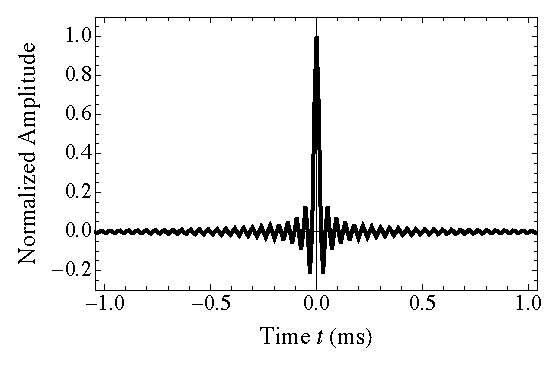
\includegraphics[width = \columnwidth]{A5_impulse_response/figures/Farina_Inverse_BPF_IR_Sm}
        \caption{Impulse response}
    \end{subfigure}
    \hfill
    \begin{subfigure}[b]{0.482\textwidth}
        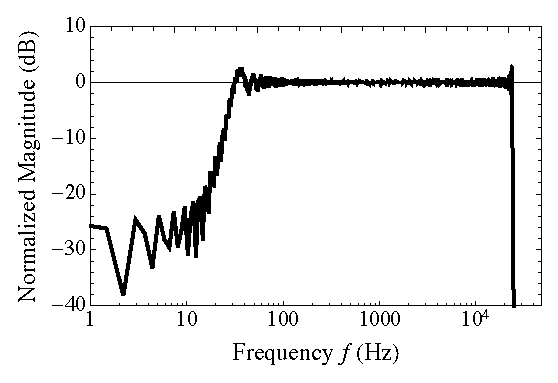
\includegraphics[width = \columnwidth]{A5_impulse_response/figures/Farina_Inverse_BPF_FR_Sm}
        \caption{Magnitude response}
    \end{subfigure}
\caption[Band-pass filter due to time-reversed deconvolution.]{
An example of the resulting band-pass filter due to time-reversed deconvolution for a $\sim23$ Hz to 24 kHz phase-controlled ESS sampled at 96 kHz.}
\label{fig:farina_BPF}
\end{figure}

For both of these deconvolution techniques, linear convolution of the recorded signal with the inverse signal is recommended to prevent part of the IR from ``wrapping around'' via cyclic convolution \citep{Farina2007a}.
The FFT can still be used, however, provided that each signal is zero-padded to at least twice its length, in which case multiplication in the frequency domain is equivalent to linear convolution in the time domain.
In our implementation, we perform exact deconvolution with appropriate zero-padding to extract the IR.

\subsection{Loudspeaker ``pop''}
One of the problems with the conventional ESS as defined in \eqnref{eq:A5_Impulse_Response:ESS} is that the loudspeaker may produce an audible ``pop'' at the end of the sweep.
This occurs when the ESS signal abruptly drops from a non-zero value to zero \citep{Farina2007a}.
The pop is undesirable as it introduces energy across the entire frequency spectrum, appearing as noise in the resulting IR.
Two solutions to this problem are to apply a time-domain fade-out to the end of the sweep \citep{Farina2007a} or to use a phase-controlled ESS up to the Nyquist frequency \citep{VetterdiRosario2011} to ensure that the sample values of the excitation signal converge more gradually towards zero.
It is worth emphasizing that the phase-controlled sweep will prevent the pop \textit{only} when terminated at the Nyquist frequency, since it is only under this condition that the samples leading up to the final sample converge towards zero.
In our implementation, we use a phase-controlled ESS and sweep up to the Nyquist frequency.

\subsection{Balancing SNR and pre-response}\label{sec:A5_Impulse_Response:Two-Step-ESS}
In view of the discussion in \secref{sec:A5_Impulse_Response:Introduction}, it is clear that knowledge of a system's pass-band may enable an improved measurement of the system's IR, as out-of-band noise may be freely attenuated via band-pass filtering without inadvertently creating a pre-response.
Motivated by this idea, a two-sweep measurement procedure was recently developed \citep{Tylka2014,Choueiri2018}, which is executed as follows:
\begin{enumerate}
\item a quick, full-band ESS is used to estimate the pass-band of the system under test,
\item a second, slower ESS through only that pass-band is used to measure the system's IR, and
\item a band-pass filter is applied to the second measurement in order to attenuate out-of-band noise.
\end{enumerate}
By matching the band-pass filter to the pass-band of the system, this method is able to attenuate out-of-band noise without introducing a significant pre-response \citep{Tylka2014}.
Additionally, the the removal of the out-of-band noise increases the overall SNR in the result of the second sweep.
In most quiet measurement environments, however, such additional steps are often unnecessary in order to achieve a reasonably high-SNR measurement without a significant pre-response.
Consequently, in our implementation, we use only single phase-controlled ESS measurements.

%\subsection{Signal-to-noise ratio}
%It has been stated that the measured SNR can be improved either by increasing the sweep duration or by averaging multiple measurements~\cite{Farina2007a,MullerMassarani2001R}.
%The latter technique, however, may lead to errors due to time-variant effects such as heating of the transducers or, in the case of outdoor measurements, wind.
%Consequently, we choose to employ a small number of longer sweeps.